\chapter{Интеркалирование графена на SiC(0001)}\label{ch:ch1}
\section{Экспериментальная часть}\label{sec:ch1/sec1}
По этой части работы опубликовано аж четыре статьи в ФТТ (и кусок моей магистерской).

Графен был выращен на карбиде кремния методом термического разложения 4H-SiC(0001) в вакууме в среде инертного газа как описано в \cite{Davydov2017}. После очистки поверхности образцов прогревом в вакууме был произведен контроль образцов. На Рис. \ref{img:leed} показаны картины дифракции медленных электронов, снятые на разных стадиях формирования интерфейса при энергии первичных электронов, равной 94 эВ. В частности, на Рис. \ref{img:leed}(а) приведена типичная картина для системы графен/SiC(0001). На ней хорошо видна структура $p(6\sqrt{3}\times6\sqrt{3})R30^o$, возникающая вследствие несовпадения периодов решеток графена и карбида кремния.  Четкость рефлексов свидетельствует о строгой согласованности пространственной ориентации решетки графена с подложкой. 
\begin{figure}[ht] 
  \center
  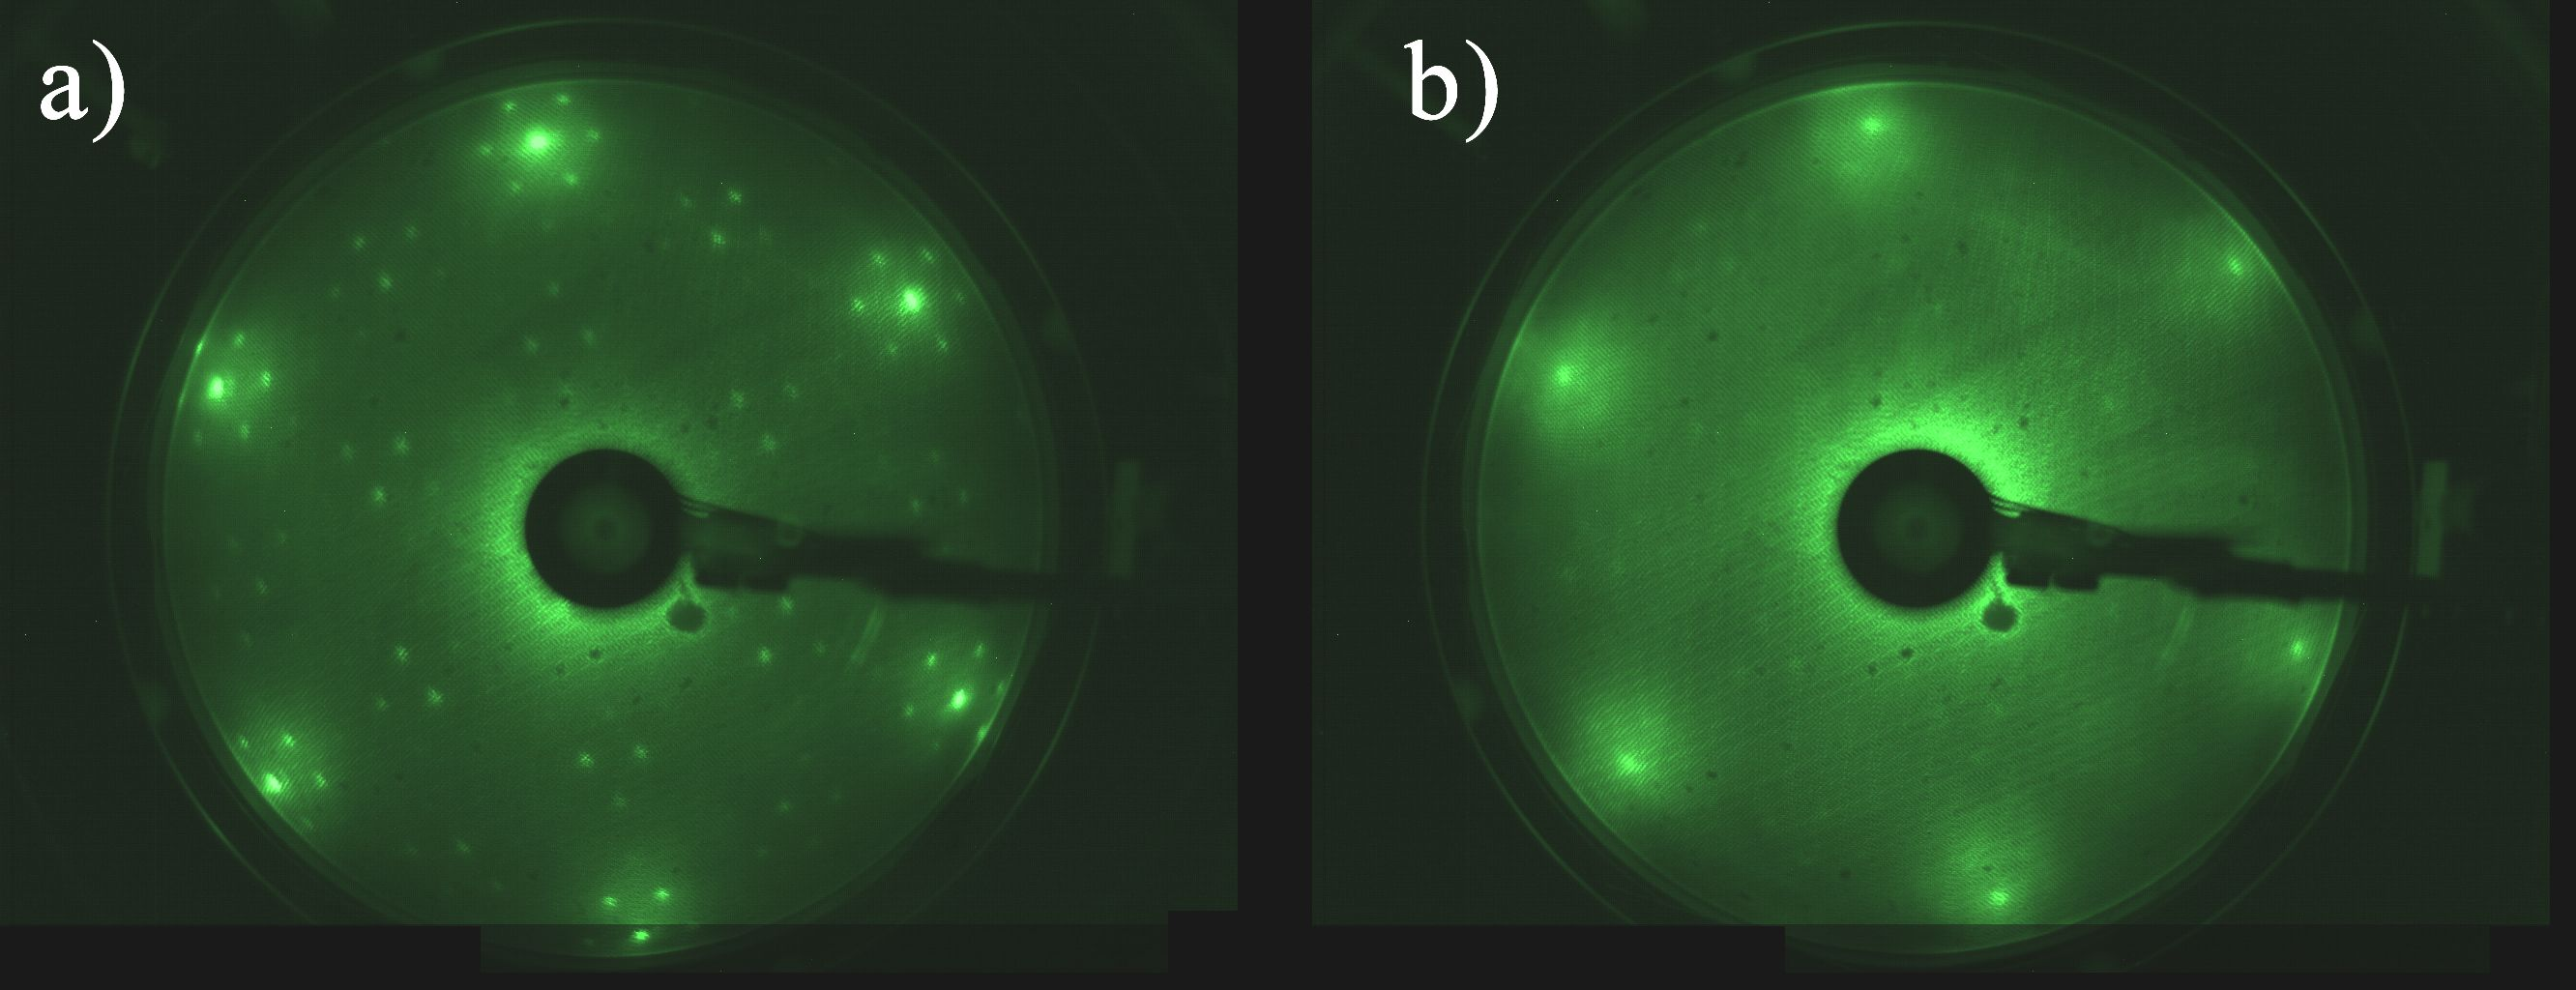
\includegraphics [scale=0.17] {fig2.jpg}
  \caption{Картины ДМЭ, полученные при энергии 94 eV: a – картина образца Gr/SiC c чистой поверхностью, b – картина, наблюдавшаяся после интеркалирования.}. 
  \label{img:leed}  
\end{figure}
%\section{Фотоэлектронная спектроскопия}
Для контроля элементного состава образцов были измерены обзорные спектры при энергии фотонов 650 eV. Они показали наличие только линий углерода и кремния, а также соответствующих пиков характеристических потерь энергии электронов. Особый интерес представляют линии С $1s$ и Si $2p$, поскольку их модификации отражают химические изменения в системе. Типичные спектры С $1s$ и Si $2p$, полученные после очистки образца, показаны на Рис. \ref{img:fig2}.

Рассмотрим результаты, полученные в ходе интеркалирования графена железом. 

Сначала железо наносилось на поверхность графена при комнатной температуре. Его напыление приводило к затуханию линий углерода и кремния (Рис. \ref{img:fig2}). После этого образец отжигали при температуре 630$^o$С. Как видно из Рис. \ref{img:fig2} (a), проведенный отжиг приводил к увеличению интенсивности графеновой компоненты линии C $1s$ до ее изначального значения. В то же время он почти не оказывал влияния на интенсивность компоненты линии C $1s$, соответствующей SiC, а также линии Si $2p$ карбида кремния (Рис. \ref{img:fig2}).  Такое поведение спектров указывает на проникновение атомов Fe в межслоевое пространство между графеном и подложкой. Протекание интеркаляции возможно благодаря доменной структуре графена: диффузионный барьер для помещенных на него атомов железа низок, и при высокой температуре атомы Fe могут мигрировать к границам доменов и проникать под графен, образуя под ним железную пленку. 
\begin{figure}[ht] 
  \center
  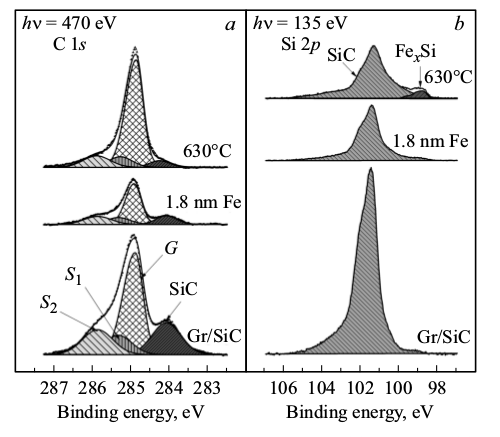
\includegraphics [scale=0.47] {fig2.png}
  \caption{Спектры фотоэлектронов C $1s$ (а) и Si $2p$ (b), измеренные для образца Gr/SiC с чистой поверхностью, после напыления на него железа и отжига при температуре 630$^o$C. }
  \label{img:fig2}  
\end{figure}
Такой вывод подкрепляется также данными, полученными методом ДМЭ. Дифракционная картина, наблюдавшаяся после интеркаляции железа, приведена на Рис. \ref{img:leed}(b). Рефлексы, соответствующие карбиду кремния, на этой картине исчезают, а остаются только рефлексы, обусловленные графеном. Однако дифракционная картина после интеркалирования графена железом становится менее четкой, диффузной, что свидетельствует о возникновении дефектов.
Следует отметить, что отжиг привел к появлению в спектре Si $2p$ новой линии с энергией связи, равной примерно 99 eV. Такие значения энергии характерны для силицидов железа \cite{Gomoyunova2010}. Причиной их возникновения является химическое взаимодействие  железа с кремнием, которое наблюдалось при температурах выше 550$^o$C. Это свидетельствует о начала разрушения подложки, поэтому в дальнейших экспериментах температура отжига была снижена. Для достижения максимальной чистоты эксперимента железо напылялось на нагретый образец. Проведенные эксперименты показали, что для активации процесса интеркаляции необходима температура выше 350$^o$C. При этом оптимальные условия  реализуются в диапазоне 400 - 500$^o$C.
\begin{figure}[ht] 
  \center
  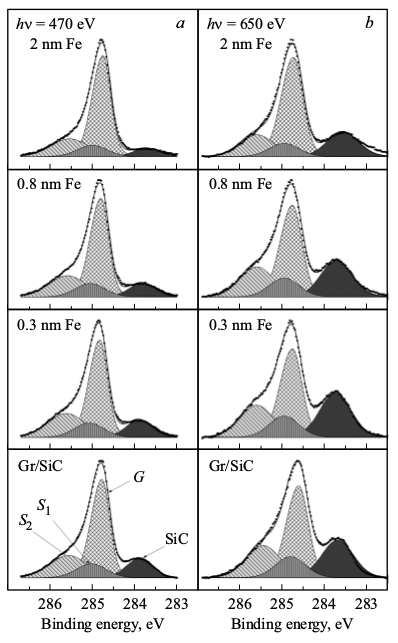
\includegraphics [scale=0.47] {fig3.png}
  \caption{Спектры C $1s$, измеренные на разных стадиях процесса }
  \label{img:fig3}  
\end{figure}

Рис. \ref{img:fig3} иллюстрирует динамику изменения формы линии С $1s$ в процессе интеркалирования графена железом при температуре 500$^o$C.Спектры снимались при энергиях фотонов 470 и 650 eV, что позволило проанализировать данные, полученные в условиях большей (470 eV) и меньшей (650 eV) поверхностной чувствительности. Из рисунка видно, что увеличение толщины слоя Fe приводит к монотонному убыванию интенсивности мод SiC и мод буферного слоя. При этом интенсивность компоненты G остается неизменной. Это свидетельствует о том, что под графеном в процессе интеркаляции вырастает пленка железа. Этот вывод подтверждается анализом картин ДМЭ.  



\begin{figure}[ht] 
  \center
  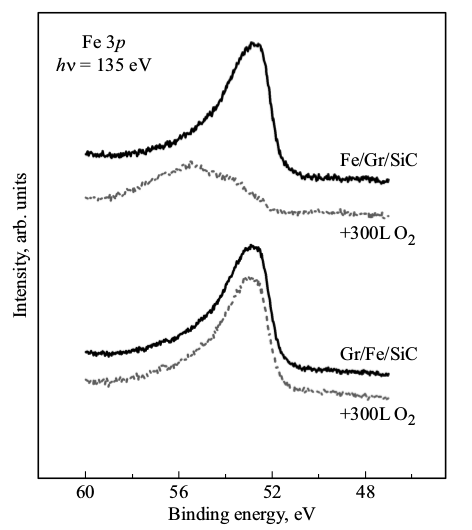
\includegraphics [scale=0.47] {gig4.png}
  \caption{Спектры Fe 3p, измеренные для систем Fe/Gr/SiC и Gr/Fe/SiC до и после их экспозиции в кислороде. }
  \label{img:fig4}  
\end{figure}
Для получения количественных данных об исследуемом процессе мы проанализировали зависимости интенсивности всех мод измеренных C1s спектров от толщины пленки железа. При этом использовалась простая модель, основанная на том, что интенсивность фотоэмиссии из каждого атомного слоя образца пропорциональна концентрации атомов в этом слое и экспоненциально затухает с глубиной в результате неупругого рассеяния электронов в вышележащем слое вещества [22]. Толщины слоев интеркалированного железа на различных стадиях процесса, оцененные по ослаблению интенсивности мод спектров углерода, приведены в таблице1. Поскольку, как уже отмечалось, с увеличением покрытия мода SiC затухает быстрее, чем моды S1 и S2, при проведении этих оценок мы учитывали возможность формирования под графеном слоев железа двух типов. Во-первых, пленки Fe, локализованной между графеном и буферным слоем (толщиной d1). Во-вторых, пленки, образующейся между буферным слоем и верхним монослоем атомов SiC(0001) (толщиной d2). Модельные расчеты, проведенные методом псевдопотенциала [9], показали, что именно эта конфигурация является энергетически наиболее выгодной для данной системы. Кроме того, в этой же работе были получены и экспериментальные данные, свидетельствующие в пользу указанного сценария процесса интеркаляции. 
Полученные нами результаты частично подтвердили этот вывод. Действительно, как видно из таблицы 1, на ранней стадии интеркалирования (после напыления 0.3 nm Fe) в приповерхностной области образца образуется лишь субмонослойная пленка железа второго типа с эффективной толщиной d2, равной 0.06nm. При этом, как показано в работе [9], контактирующие с железом участки буферного слоя трансформируются в слой графена. Однако при дальнейшем увеличении количества нанесенного железа рост этой пленки замедляется, и атомы Fe начинают накапливаться между исходным графеном и буферным слоем. В итоге после напыления 2 nm Fe на поверхности SiC образуется слоистая структура, состоящая из графена и двух слоев железа (0.31 и 0.28 nm). 
Сходный сценарий процесса интеркалирования характерен и для случая более низких температур. В качестве примера в таблице 2 представлены результаты обработки экспериментов, проводившихся при температуре 400С. Сравнение данных, приведенных в таблицах, обнаруживает их значительное сходство. Однако имеются и некоторые различия. Во-первых, при 400С формирование слоя интеркалированного железа суммарной толщиной 0.6nm достигается при существенно меньших дозах напыления Fe (1.2 nm вместо 2 nm). Во-вторых, образование пленки железа между графеном и буферным слоем идет менее активно, чем при температуре 500С. Таким образом, варьируя температуру процесса, можно, по-видимому, менять соотношение толщин d1  и d2 слоев интеркалированного железа.

Практическое использование тонких пленок железа значительно затрудняется их легкой окисляемостью на воздухе. Учитывая химическую пассивность графена, можно ожидать, что в сформированной интеркаляционной системе Gr/Fe/SiC слои железа защищены графеном от воздействия кислорода. Для проверки правильности этого вывода был проведен специальный эксперимент. В ходе его в условиях сверхвысокого вакуума на поверхность двух идентичных образцов графен/4Н-SiC(0001) было нанесено железо. При этом первый образец находился при комнатной температуре, а температура второго поддерживалась равной 450$^o$C. Это должно было обеспечить формирование пленки железа на графене в случае первого образца и пленки железа под графеном для второго. Спектры Fe $3p$ электронов, измеренные после напыления Fe, показаны на Рис. \ref{img:fig4}. Далее каждый из этих образцов был подвергнут выдержке в атмосфере кислорода при давлении $10^{-6}$ mbar и комнатной температуре с общей экспозицией 300 L. После чего были вновь измерены те же спектры. Видно, что воздействие кислорода оказало сильное влияние на  линию Fe $3p$ первого образца. Она изменила свою форму и испытала химический сдвиг, демонстрирующий образование оксидов железа. В случае же второго образца практически никаких изменений спектра не наблюдалось, и графен, действительно, воспрепятствовал окислению сформированной пленки. Следует также отметить, что этот эксперимент убедительно доказывает факт формирования интеркаляционной системы графен/Fe/SiC, а также свидетельствует о достаточно высоком качестве графена. 

\begin{figure}[ht] 
  \center
  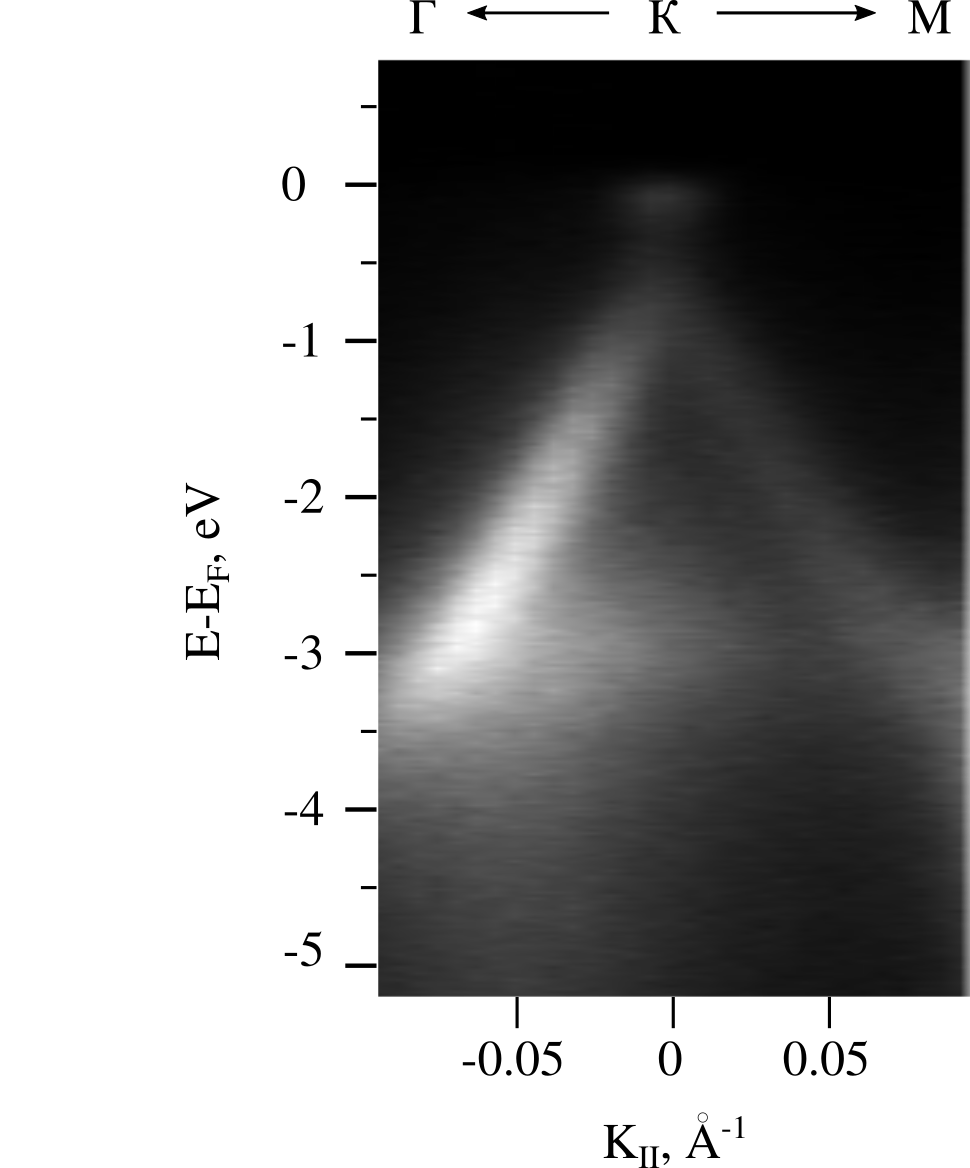
\includegraphics [scale=1] {fig103.png}
  \caption{Спектр ФЭСУР, полученный для системы графен/Fe/SiC(0001). }
  \label{img:fig6}  
\end{figure}

Для исследования электронной структуры полученной системы с одного из образцов был снят спектр ФЭСУР валентной зоны в окрестности точки К зоны Брюллюэна, представленный на Рис. \ref{img:fig6}. На нем видно ключевую особенность зонной структуры графена - конус Дирака. Конус Дирака оказывается смещен в сторону больших энергий связи на 0.4 eV, что показывает слабое n-допирование графена, вызванное взаимодействием с подложкой. Железо - металл с незаполненной d-оболочкой. Его присутствие между буферным слоем и подложкой проявляется в возникновении гибридных орбиталей, образующихся при перекрытии $p_z$ орбиталей атомов углерода буферного слоя и $3d$ орбиталей атомов железа. На спектре ФЭСУР гибридное состояние находится при энергии связи -3 eV.

%\section{Ближняя тонкая структура рентгеновских спектров поглощения}

В качестве примера на рис. 5 представлены массивы спектров КРС для образца до и после интеркалирования железом (2 nm Fe, 500C). Спектры получены после вычитания мешающего вклада спектра подложки 4H-SiC. Измерения были выполнены на площади 20 × 20 мкм с шагом 2 микрона. Количество спектров в каждом массиве (N) равно 124. В спектрах наблюдаются особенности, возникающие при рассеянии света от графеновой пленки: линии G, 2D и D [23]. На рис. 6 приведено сравнение типичных спектров содержащихся в массивах спектров КРС, представленных на рис. 5,а и 5,b. Видно, что в результате интеркалирования происходит низкочастотный сдвиг линий G и 2D в спектре и их уширение, а также сильно увеличивается интенсивность линии D. Следует отметить, что положение линии G в обоих спектрах регистрируется на частотах имеющих более высокие значения, чем частота ω=1580 см−1, характерная для объемного кристаллического графита. Причиной этого могут быть два фактора: деформация сжатия вдоль слоя, которая возникают вследствие разницы коэффициентов термического расширения решетки графена и SiC, и/или избыток заряда по сравнению с электрически нейтральным графеном [24-26]. Одним из способов, позволяющих разделить вклады деформации и изменения зарядового состояния, является совместный анализ положения линий G и 2D [27]. В этой работе была установлена зависимость между положениями G и 2D линий для электрически нейтрального графена в условиях двуосной деформации: 
ω2D = 2671 + 2.8(ωG − 1581) см−1.                              %                                           (1) 
На вставке к рис. 6 представлены данные о корреляции между положениями линий 2D и G в спектрах исходного образца и образца, подвергнутого интеркалированию. Эти данные были полученные в результате обработки соответствующих массивов спектров, представленных на рис. 5,а и 5,b. Хорошее согласие экспериментальных данных с зависимостью (1) указывает на то, что положение фононных линий в спектрах обоих образцов преимущественно обусловлено наличием деформации, при этом ее величина меньше в образце подвергнутом интеркалированию.
С использованием данных работы [27], средняя величина деформации сжатия в плоскости слоя для исходного образца может быть оценена как ǀǀ= (0.37±0.04)\% из сдвига ωG = 23 см-1. Разброс величины в пределах 10\% говорит о наличии не очень большой локальной неоднородности в распределении деформации в образце. В то же время средняя величина деформации сжатия в плоскости слоя для образца, подвергнутого интеркалированию железом, существенно меньше и может быть оценена как ǀǀ= (0.11±0.09)\% из сдвига ωG = 7 см-1. Однако разброс величины в пределах 90\% указывает на очень существенную неоднородность в распределении деформации по анализируемой площади образца, что может быть также причиной наблюдаемого значительного уширения фононных линий в его спектре. 
По сравнению со спектром КРС исходного графенового слоя для спектра образца интеркалированного железом характерно существенное увеличение интенсивности D-полосы. Известно, что отношение интегральных интенсивностей двух полос (ID/IG) является мерой степени беспорядка и обратно пропорционально среднему размеру sp2-кластеров [28, 29]. Увеличение этого параметра в спектре интеркалированного образца указывает на его большую дефектность и уменьшение размера sp2-кластеров в нем по сравнению с исходным графеновым слоем. Так, концентрацию дефектов в кристаллической решетке исходного образца можно оценить как Nd < 1010 сm-2, тогда как для интеркалированного образца она близка к Nd ~ 1012 сm-2 [26]. 
Несмотря на высокую концентрацию дефектов, образовавшихся в графене при его интеркалировании железом, электронная структура этого двумерного материала сохранила свои ключевые особенности. Об этом свидетельствуют результаты, полученные методом спектроскопии рентгеновского поглощения вблизи K-края углерода. Соответствующие данные приведены на Рис. \ref{img:fig7}, на котором показаны две пары спектров ближней тонкой структуры рентгеновских спектров поглощения (NEXAFS), измеренных до и после интеркалирования образца железом. При измерениях использовалась задерживающая сетка с потенциалом –200 V, отсекающая медленные электроны, выходящие преимущественно из объема SiC. Это обеспечивало высокую поверхностную чувствительность спектров и доминирующий вклад в них графена и буферного слоя. 
\begin{figure}[ht] 
  \center
  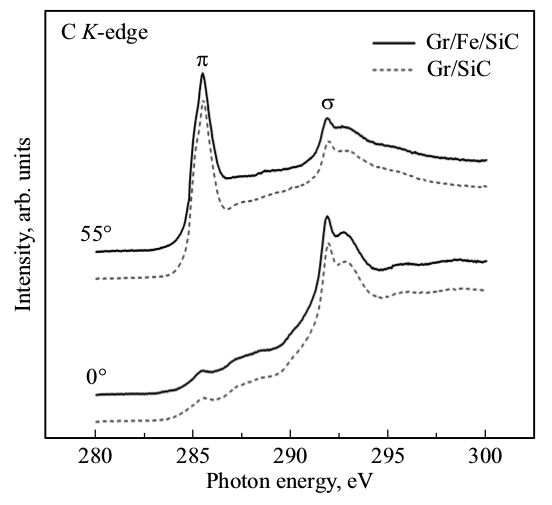
\includegraphics [scale=0.37] {fig7.png}
  \caption{Спектры NEXAFS, измеренные до и после интеркалирования образца железом. Углы между плоскостью образца и вектором поляризации падающего излучения указаны возле кривых. }
  \label{img:fig7}  
\end{figure}

Характерной особенностью спектров поглощения графеноподобных структур является наличие $\pi$- и $\sigma$-резонансов, имеющих противоположные угловые зависимости. Максимальная интенсивность $\sigma$-резонанса должна наблюдаться в случае, когда вектор поляризации излучения лежит в плоскости графена (0$^o$). При этом интенсивность $\pi$-резонанса должна быть, наоборот, минимальной. Именно такая угловая зависимость интенсивности пиков $\pi$ и $\sigma$ наблюдается на Pис. \ref{img:fig7} для исходного образца. Это свидетельствует о том, что как графен, так и буферный слой являются планарными $sp2$ структурами, ориентированными параллельно поверхности SiC(0001). Видно, что процесс интеркалирования, действительно, практически не оказал никакого влияния на вид кривых. Это свидетельствует о том, что графен сохранил свою планарную структуру.


\section{Теоретическая часть}\label{sec:ch1/sec1}
По теоретической части есть статья в конференционном журнале и еще одна в ФТТ (ее планируется подать до конца года).
